\documentclass[a4paper, 12pt]{paper}

\usepackage[utf8]{inputenc}
\usepackage[T1]{fontenc}

% Quelques packages utiles
\usepackage{listings} % Pour afficher des listings de programmes
\usepackage{graphicx} % Pour afficher des figures
\usepackage{amsthm}   % Pour créer des théorèmes et des définitions
\usepackage{amsmath}
\usepackage{amssymb}
\usepackage{url}
\usepackage{booktabs} % Allows the use of \toprule, \midrule and \bottomrule in tables for horizontal lines
\usepackage[per-mode=symbol]{siunitx}
\usepackage{floatrow}  
\usepackage[justification=centering]{caption}
\usepackage{subcaption}
\usepackage{fullpage}
\usepackage{lipsum}
\usepackage{cite}
\usepackage{numprint}
\usepackage{hyperref}
\usepackage{here}

\author{Florian Reinhard\\
        \texttt{florian.reinhard@epfl.ch} \and
        Pius von Däniken\\
        \texttt{pius.vondaeniken@epfl.ch}}

\title{Laser beacons and dead reckoning}

\begin{document}

\maketitle

\tableofcontents

\section{Introduction}

\subsection{The Problem}

We want to calculate the position of a moving robot in a 2D plane by measuring
the relative angles between three beacons with known coordinates.
As we don't measure the absolute angles to some fixed direction (like north in
nautical bearing~\cite{wikipedia_bearing}), we absolutely need all three
angles to calculate the Cartesian coordinates of our robot.

If the position of the three beacons and the robot all lie on a circle, the
fact that the transformation from the measured angles to the coordinates is not
\emph{injective}, starts to present a problem as described in
Section~\ref{ss2:algorithm} and shown in Figure~\ref{fig:error_map}.

\begin{figure}[H]
    \centering
    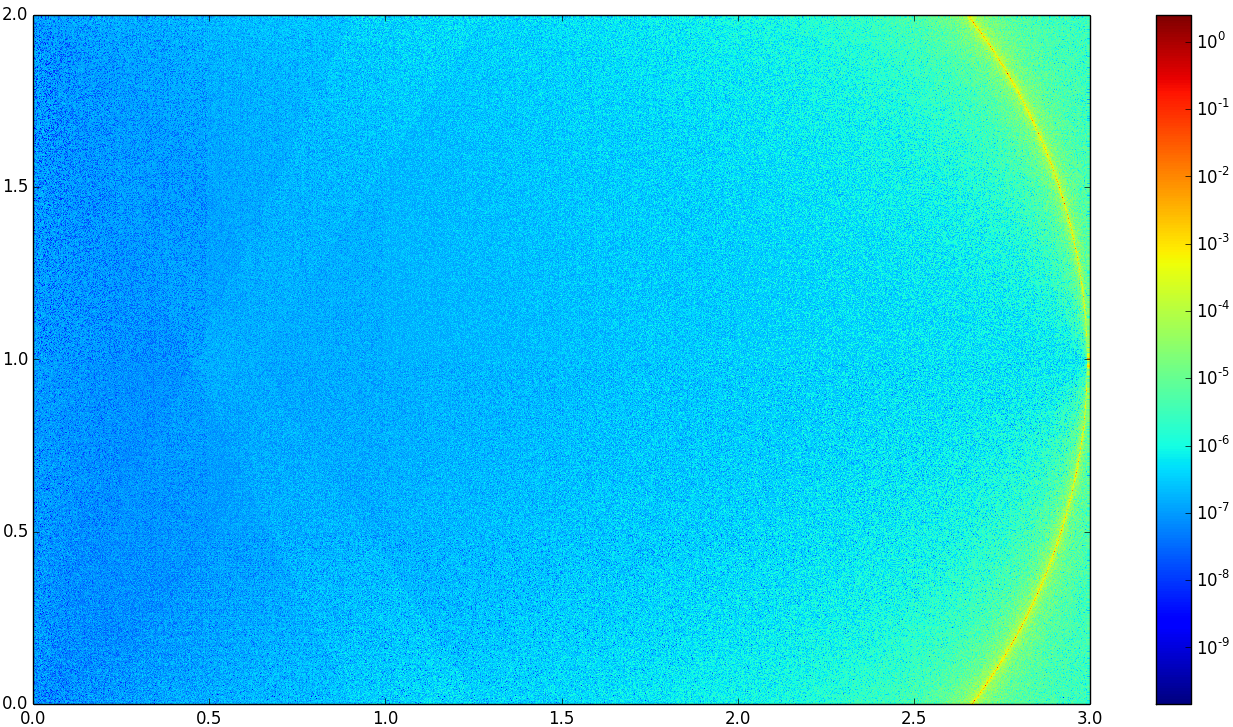
\includegraphics[width=\textwidth]{error_color_map_log}
    \caption{Representation of the magnitude of the error due to
        \emph{floating point errors} errors when calculating the position from
        the measured angles. Every pixel represents a position that has been
        transformed into the angles that should have been measured and then back
        into cartesian coordinates. The \emph{beacons} are positioned at
        $\left(0, 0\right)$, $\left(0, 2\right)$, and $\left(3, 1\right)$}
\label{fig:error_map}
\end{figure}

\subsection{Positioning with beacons}

We measure the angles $x$, $y$, and $z$ and we want to calculate the vector $P$.
It seems like a logical conclusion to use a
\emph{barycentric coordinate system}~(\ref{ss2:bary}) to solve this problem.


\subsubsection{Barycentric coordinates}
\label{ss2:bary}

In a two-dimensional barycentric coordinate system a position is specified as
the center of mass of masses placed at the vertices of a triangle. In our case
the vertices are at the beacons' positions.

\begin{figure}[H]
    \centering
    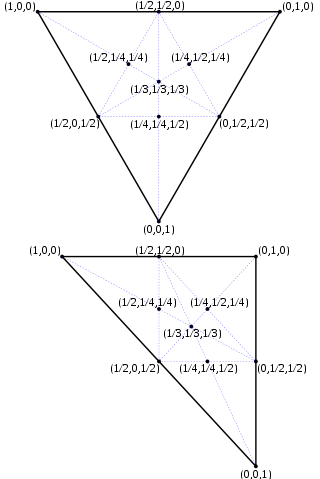
\includegraphics[width=0.5\textwidth]{bary}
    \caption{Several points in different barycentric coordinate systems.}
\label{fig:bary}
\end{figure}

\subsubsection{The algorithm}
\label{ss2:algorithm}

The \emph{barycentric coordinates} of $P$ in figure~\ref{fig:three_angles} are
\begin{equation}
    \left(\frac{1}{\cot{A} - \cot{x}} :
          \frac{1}{\cot{B} - \cot{y}} :
          \frac{1}{\cot{C} - \cot{z}} \right)
    \label{eq:p}
\end{equation}
where $A$, $B$, and $C$ are the triangle's angles at the corresponding
vertices~\cite{bary_coordinates_formula}.

If now $P$ lies on the circle going through $A$, $B$, and
$C$ (figure~\ref{fig:p_on_circle}), we have the problem that two of the three coordinates
in equation~\ref{eq:p} are equal to $\frac{1}{0}$ and thus tend to infinity.
On top of that, the coordinates are constant per segment between vertices (this
can be explained by the
\emph{inscribed angle theorem}~\cite{wikipedia_inscribed_angle}).

\begin{figure}[H]
    \centering
    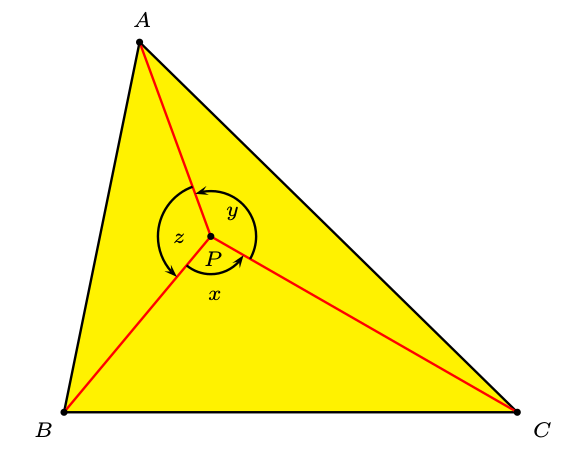
\includegraphics[width=0.7\textwidth]{three_angles}
    \caption{The three angles that are measured when positioning with beacons.}
\label{fig:three_angles}
\end{figure}

\begin{figure}[H]
    \centering
    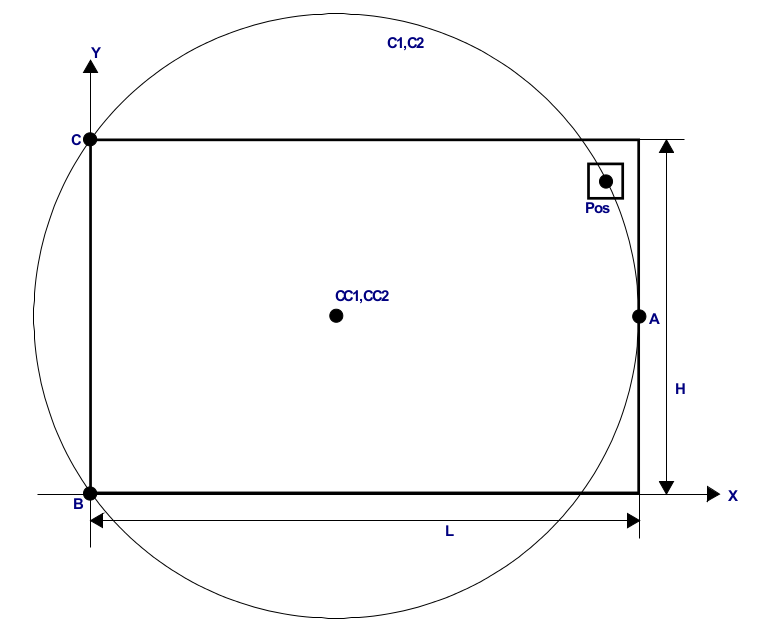
\includegraphics[width=0.8\textwidth]{p_on_circle}
    \caption{$P$ lies on the circle going through $A$, $B$, and $C$.}
\label{fig:p_on_circle}
\end{figure}

\subsection{Dead reckoning}

\emph{Dead reckoning} is the process of deducing the current position off of a
previously determined position and the advanced distance based upon known or
estimated speeds over elapsed time and course.~\cite{wikipedia_dead_reckoning}

\subsection{Kalman Filter}

Here is just the algorithm adapted to our needs. Maybe start with
\emph{wikipedia}~\cite{wikipedia_lqe} for actual explanations.

\paragraph{Predict}

\begin{equation}
    \mathbf{\hat{x}}_k = \mathbf{F}_k \mathbf{{x}}_{k-1}
\label{eq:state_predict}
\end{equation}

$\mathbf{\hat{x}}_k$ is the new \emph{prediction} of the state,
$\mathbf{F}_k$ and $\mathbf{{x}}_{k-1}$ are the \emph{state transition matrix}
and the old state estimation.

\begin{equation}
    \mathbf{\hat P}_k = \mathbf{F}_k \mathbf{P}_{k-1} \mathbf{F^T}_k + \mathbf{Q}_k
\label{eq:cov_predict}
\end{equation}

The covariance $\mathbf{\hat P}_k$ of the predicted state depends on the previous
covaraiance, the state transition function and the \emph{state transition error}
$\mathbf{Q}_k$ (see~\ref{pg:variance_state_trans}).

\paragraph{Update}

\begin{equation}
    \mathbf{y}_k = \mathbf{z}_k - \mathbf{H}_k \mathbf{\hat x}_k
\label{eq:measurement_residual}
\end{equation}

$\mathbf{y}_k$ is the \emph{measurement residual}, $\mathbf{z}_k$ is the measurement,
and $\mathbf{H}_k$ transforms the state in to \emph{measurement space}. (Note that
we don't have a control.)

\begin{equation}
    \mathbf{S}_k = \mathbf{H}_k \mathbf{P}_k \mathbf{H^T}_k + \mathbf{R}_k
\label{eq:residual_cov}
\end{equation}

$\mathbf{S}_k$ is the \emph{residual covariance} and $\mathbf{R}_k$ is the covariane
of the measurement's \emph{noise}.

\begin{equation}
    \mathbf{K}_k = \mathbf{P}_k \mathbf{H^T}_k \mathbf{S^{-1}}_k
\label{eq:kalman_gain}
\end{equation}

$\mathbf{K}_k$ is the \emph{Kalman gain}.

\begin{equation}
    \mathbf{x}_k = \mathbf{\hat x}_k + \mathbf{K}_k \mathbf{y}_k
\label{eq:updated_extimate}
\end{equation}

$\mathbf{x}_k$ is the \emph{updated state estimation}.

\begin{equation}
    \mathbf{P}_k = \left( \mathbf{I} - \mathbf{K}_k \mathbf{H}_k \right) \mathbf{P}_k
\label{eq:updated_cov}
\end{equation}

$\mathbf{P}_k$ is the \emph{updated estimate covariance}.

\section{Adding dead reckoning to the game}

\subsection{Why?}

Because of the enormous error of the beacon system at certain positions and the
high probability of outages (another robot obstructing the line of sight), a
\emph{Kalman filter} integrating dead reckoning and the beacons should increase
the precision and usability of the system.

\subsection{Kalman Filter}
\paragraph{State variables}

A possible state for the Kalman filter is

\begin{equation}
    \mathbf{x_k} = \left( \begin{array}{c} x_k     \\
                                           y_k     \\
                                           x_{k-1} \\
                                           y_{k-1} \end{array} \right)
\label{eq:kalman_state}
\end{equation}

\paragraph{State transition}

\begin{equation}
    \mathbf{F_k} = \left( \begin{array}{cccc} 1 + \tau & 0 & -\tau & 0\\
                                              0 & 1 + \tau & 0 & -\tau\\
                                              1 & 0 & 0 & 0 \\
                                              0 & 1 & 0 & 0 \end{array} \right)
\label{eq:state_trans}
\end{equation}

Where $\tau$ is the factor $ \frac{t_k - t_{k-1}}{t_{k-1} - t_{k-2}}$.
This makes for the following computation:
\begin{equation}
    \mathbf{x_k} = \mathbf{x_{k-1}} + \mathbf{\Delta x_k}
    = \mathbf{x_{k-1}} + \mathbf{v_{k-1}} \Delta t_k
    = \mathbf{x_{k-1}} + \frac{\mathbf{x_{k-1}} - \mathbf{x_{k-2}}}
                              {\Delta t_{k-1}} \Delta t_k
\label{eq:state_trans_math}
\end{equation}

\paragraph{Measurement}

\begin{equation}
    \mathbf{H} = \left( \begin{array}{cccc} 1 & 0 & 0 & 0\\
                                            0 & 1 & 0 & 0 \end{array} \right)
\label{eq:h}
\end{equation}

Not much to say about that.

\subsubsection{Variances}

\paragraph{For the state transition}
\label{pg:variance_state_trans}
we can safely assume that almost $100\%$ of the time, the robot
won't accelerate more than the maximal acceleration which our regulation will
use (only collisions and such can make the robot to accelerate more).
For a \emph{gaussian distribution}, $99.8\%$ are inside $4\sigma$, so we say
that $4\sigma = \frac{1}{2} a_{\max} {\left( t_k - t_{k-1} \right)}^2 $ and thus 
$\sigma = \frac{1}{8} a_{\max} {\left( t_k - t_{k-1} \right)}^2 $ is the standard
deviation of our control update i.e. $\mathbf{Q}$.

\begin{equation}
    \mathbf{Q_k} = \left( \begin{array}{cccc}
        \frac{1}{64} a_{\max}^2 \Delta t^4 & \frac{1}{64} a_{\max}^2 \Delta t^4 & 0 & 0\\
        \frac{1}{64} a_{\max}^2 \Delta t^4 & \frac{1}{64} a_{\max}^2 \Delta t^4 & 0 & 0\\
        0 & 0 & 0 & 0 \\
        0 & 0 & 0 & 0 \end{array} \right)
\label{eq:q}
\end{equation}

\paragraph{The measurement}'s variance will have to determined experimentally
and should be adapted when the robot approaches the \emph{circle of death}.


\section{Results and expectations}

\emph{To be done.}


\bibliographystyle{abbrv}
\bibliography{beacons_with_kalman}
\end{document}
